%!TEX root = /Users/mn/Developer/working-copies/smalltalks/dancinglinksst/ESUG2019/esug.tex

\documentclass[10pt]{beamer}


\usepackage[utf8x]{inputenc}
\usepackage[T1]{fontenc}
\usepackage{textcomp}
\usepackage{minted}
\usepackage[scaled=0.8]{beramono}
\usepackage{amsmath}
\usepackage{amsthm}
\usepackage{amssymb}
\usepackage{euler}
\usepackage{fancyvrb}

\usefonttheme[onlymath]{serif}

\usemintedstyle{friendly}

\setbeamertemplate{blocks}[rounded]

%Information to be included in the title page:
\title{Dancing Links\\\small{an educational pearl}}
\author{Massimo Nocentini, PhD.\\\footnotesize{massimo.nocentini@gmail.com}}
\institute{ESUG2019 -- \today.}
\date{\vspace{0.5cm}
\includegraphics{SchmidtLogo.jpg}}

\begin{document}

\frame{\titlepage}

\logo{
\includegraphics[height=0.5cm,width=3cm]{SchmidtLogo.jpg}\vspace{240pt}}

\begin{frame}[fragile]
\frametitle{}
\begin{minted}[fontsize=\small]{smalltalk}
outline
    ^ LinkedList new
        add: 'me and the core idea';
        add: 'DoubleLink objs';
        add: 'exact cover problem';
        add: 'AlgorithmX';
        add: 'covering and uncovering columns';
        add: 'N-Queens and Sudoku problems';
        yourself
\end{minted}
\end{frame}

\begin{frame}[fragile]
\frametitle{Hi!}
\begin{Verbatim}[fontsize=\small]
$ whoami
Massimo Nocentini, PhD
Mathematician (algebraic combinatorics, formal methods for algs)
Programmer (automated reasoning, logics and symbolic computation)
https://github.com/massimo-nocentini/dancinglinksst
\end{Verbatim}
\vfill
In Donald's words\footnote{\url{https://arxiv.org/abs/cs/0011047}\\Donald Knuth's 24th Annual Christmas Lecture (\url{https://youtu.be/_cR9zDlvP88})}:
\emph{
Suppose $x$ points to an element of a doubly linked list;
let $L[x]$ and $R[x]$ point to the predecessor and successor
of that element. Then:
\begin{displaymath}
  L[R[x]] \leftarrow L[x],\quad R[L[x]] \leftarrow R[x] \quad(1)
\end{displaymath}
remove $x$ from the list; every programmer knows this.
But comparatively few programmers have realized that
\begin{displaymath}
  L[R[x]] \leftarrow x,\quad R[L[x]] \leftarrow x \quad(2)
\end{displaymath}
will put $x$ back again, without references to the whole list at all.
}

\end{frame}

\begin{frame}[fragile]
\frametitle{Main ideas}

\begin{itemize}
  \item Operation $(2)$ arises in \textbf{backtrack programs}, which enumerate all 
  solutions to a given set of constraints and it was introduced in 1979 by Hitotumatu and Noshita.
  \item The beauty of $(2)$ is that operation $(1)$ can be undone by knowing only the value of $x$.
  \item We can apply $(1)$ and $(2)$ repeatedly in complex data structures that involve large 
  numbers of interacting doubly linked lists.
  \item Knuth: ``\emph{This process causes the pointer variables inside the global data structure to execute an 
    exquisitely choreographed dance; hence I like to call $(1)$ and $(2)$ the \textbf{technique of dancing links}.}''
  \item Knuth's AlgorithmX is a dedicated algorithm that can find all exact covers;
  	it is a simple depth-first backtracking-based search algorithm that runs
	efficiently via $(1)$ and $(2)$.
  \item Minato et al. \footnote{\url{https://aaai.org/ocs/index.php/AAAI/AAAI17/paper/view/14907}} 
  represent the set of sols using Zero-suppressed BDD (ZDD) that enables the efficient 
  use of memo caching to speed up the search.
\end{itemize}
\end{frame}

\begin{frame}[fragile]
\frametitle{\texttt{DoubleLink}s and \texttt{DoubleLinkedList}s}
\texttt{DoubleLink} objects respond to messages
\begin{minted}[fontsize=\small]{smalltalk}
remove
  nextLink ifNotNil: [ :next | next previousLink: previousLink ].
  previousLink ifNotNil: [ :previous | previous nextLink: nextLink ]
\end{minted}
and
\begin{minted}[fontsize=\small]{smalltalk}
restore
  nextLink ifNotNil: [ :next | next previousLink: self ].
  previousLink ifNotNil: [ :previous | previous nextLink: self ]
\end{minted}
that implement operations $(1)$ and $(2)$, respectively;
moreover, we extend \texttt{DoubleLinkedList} objects with the message
\begin{minted}[fontsize=\small]{smalltalk}
makeCircular
  head
    ifNotNil: [ 
      head previousLink: tail.
      tail nextLink: head ]
\end{minted}
to introduce circular, doubly connected, lists.
\end{frame}

\begin{frame}[fragile]
\frametitle{Exact Cover $\in \mathcal{NP}$}
\emph{Given a matrix of $0$s and $1$s, does it have a set of rows containing \textbf{exactly one} symbol $1$ in each column?}
\begin{columns}
     \begin{column}{.7\linewidth}
      Let $r_{i}\in\lbrace 0, 1 \rbrace$, the matricial equation
      \begin{displaymath}
        \left(\begin{array}{c}
          r_{1} \\ r_{2} \\ r_{3} \\ r_{4} \\ r_{5}
        \end{array}\right)^{T}
        \left(\begin{array}{cccccc}
          1 & 1 & 1 & 0 & 1 & 0 \\
          1 & 1 & 0 & 0 & 0 & 0 \\
          0 & 0 & 0 & 1 & 0 & 1 \\
          0 & 0 & 1 & 1 & 0 & 1 \\
          0 & 0 & 1 & 0 & 1 & 0 \\
        \end{array}\right) = 
        \left(\begin{array}{c}
          1 \\ 1 \\ 1 \\ 1 \\ 1 \\ 1
        \end{array}\right)^{T}
      \end{displaymath}
      is solved by two sets of rows, namely 
      $\left\lbrace r_{1}=1, r_{3}=1\right\rbrace$ and
      $\left\lbrace r_{2}=1, r_{5}=1, r_{3}=1\right\rbrace$.
     \end{column}
     \begin{column}{.3\linewidth}
       \begin{tabular}{cc}
          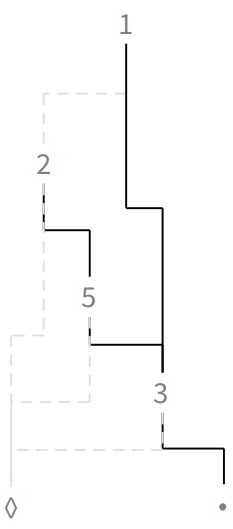
\includegraphics[width=3cm,height=5cm]{ZDD.png}
       \end{tabular}
     \end{column}
   \end{columns}
We can think of the columns as elements of a universe, and the rows as subsets of the universe; 
then the problem is to cover the universe with disjoint subsets, $\mathcal{NP}$-complete even 
when each row contains exactly three $1$s.
\end{frame}

\begin{frame}[fragile]
\frametitle{AlgorithmX}
AlgorithmX finds all sols to the Exact Cover problem defined by any given matrix A of 0s and 1s. It is simply a statement of the obvious trial-and-error approach\footnote{"Indeed, I can’t think of any other reasonable way to do the job, in general."} and can now be cast in the following explicit, deterministic recursive procedure \verb|search(k)|, which is invoked initially with \verb|k = 0|:
\vfill
\begin{Verbatim}[fontsize=\small]
if R[h] = h, print the current solution and return;
	otherwise, choose a column object c.
Cover column c.
For each r ← D[c], D[D[c]], ... while r ≠ c,
	cover column j;
search(k + 1);
set r ← O[k] and c ← C[r];
for each j ← L[r], L[L[r]], ... while j ≠ r,
	uncover column j.
Uncover column c and return.
\end{Verbatim}
\end{frame}

\begin{frame}[fragile]
\frametitle{AlgorithmX}
\begin{itemize}
	\item DLX has been empirically confirmed to be the fastest for solving exact covers
		\footnote{Junttila, T., and Kaski, P. 2010. Exact cover via satisfiability: An empirical study.}.
	\item Exact covers allow maximization of a complex objective function.
	\item Design of combinatorial objects like electric circuits and tiling problems (tetrasticks, parallelogram polyominoes, board games, ...).
	\item Since DLX is a depth-first-search-based method, it may encounter the same sub-problems several times.
	\begin{itemize}
		\item ZDDs that contain solutions to sub-problems, sub-ZDDs (subgraphs), memo cache only requires constant memory for each problem by storing the address of the root node of the sub-ZDD representing the set of solutions.
		\item ZDDs support operations that can run in time proportional to ZDD size; for example, model counting, enumeration of subsets and efficient binary operations over families of sets.
	\end{itemize}
\end{itemize}
\end{frame}

\begin{frame}[fragile]
\frametitle{AlgorithmX instance side}
\begin{minted}[fontsize=\small]{smalltalk}
searchDepth: k forDLRootObject: h partialSelection: cont
  ^ (h isFixPointOf: [ :ro | ro right ])
      ifTrue: [ self yieldNode: top onBlock: cont ]
      ifFalse: [ 
        memo
          at: h columns
          ifPresent: [ :tree | self yieldNode: tree onBlock: cont ]
          ifAbsentPut: [ 
            self
              searchDepth: k
                forDLColumnObject: h chooseColumn
                partialSelection: cont ] ]
\end{minted}
\end{frame}

\begin{frame}[fragile]
\frametitle{AlgorithmX instance side}
\begin{minted}[fontsize=\small]{smalltalk}
searchDepth: k forDLColumnObject: c partialSelection: sel
  ^ self
      onEnter: [ c cover ]
      do: [ 
        c
          untilFixPointOf: [ :co | co up ]
          foldr: [ :r :x | 
            | y |
            y := self searchDepth: k 
                        forDLDataObject: r 
                        partialSelection: sel.
            y isZDDBottom
                ifTrue: [ x ]
                ifFalse: [ 
                  self
                    uniqueNodeWithDLDataObject: r
                      withLowerNode: x
                      withHigherNode: y ] ]
          init: bottom ]
      onExit: [ c uncover ]
\end{minted}
\end{frame}

\begin{frame}[fragile]
\frametitle{AlgorithmX instance side}
\begin{minted}[fontsize=\small]{smalltalk}
searchDepth: k forDLDataObject: r partialSelection: cont
  ^ self
      onEnter: [ r untilFixPointOf: [ :ro | ro right ] 
                   do: [ :j | j column cover ] ]
      do: [ self
              searchDepth: k + 1
                forDLRootObject: r column root
                partialSelection: [ :sel | 
                  cont
                    value:
                      (ValueLink new
                        value: r model;
                        nextLink: sel;
                        yourself) ] ]
      onExit: [ r untilFixPointOf: [ :ro | ro left ] 
                  do: [ :j | j column uncover ] ]
\end{minted}
\end{frame}

\begin{frame}[fragile]
\frametitle{AlgorithmX instance side}
The entry point is the message
\vfill
\begin{minted}[fontsize=\small]{smalltalk}
searchDLRootObject: h onSolutionDo: aBlock
  ^ self
      searchDepth: 0
      forDLRootObject: h
      partialSelection: [ :selLink | 
        aBlock value: (LinkedList new add: selLink; asSet) ]
\end{minted}
\vfill
Knuth advices to use the heuristic (provided by \texttt{DLRootObject} objs)
\begin{minted}[fontsize=\small]{smalltalk}
chooseColumn
  ^ self chooseColumnWithWeight: #size withOpt: #<
\end{minted}
\begin{minted}[fontsize=\footnotesize]{smalltalk}
chooseColumnWithWeight: weightBlock withOpt: optBlock
  ^ self
      untilFixPointOf: [ :ro | ro left ]
      foldr: [ :j :r | 
        (optBlock value: (weightBlock value: j) value: (weightBlock value: r))
          ifTrue: [ j ]
          ifFalse: [ r ] ]
      init: self right
\end{minted}
that \textit{minimizes} the search tree's branching factor.
\end{frame}

\begin{frame}[fragile]
\frametitle{DLColumnObject instance side}
The operation of \emph{covering} column $c$ removes $c$ from the header list and removes all rows in $c$'s own list from the other column lists they are in.
\vfill
\begin{minted}[fontsize=\small]{smalltalk}
cover
  we remove.
  self
    untilFixPointOf: [ :co | co down ]
    do: [ :i | 
      i
        untilFixPointOf: [ :do | do right ]
        do: [ :j | 
          j nsLink remove.
          j column updateSize: [ :s | s - 1 ] ] ]
\end{minted}
\vfill
Operation $(1)$ is used here to remove objects in both the horizontal and vertical directions.
\end{frame}

\begin{frame}[fragile]
\frametitle{DLColumnObject instance side}
Finally, we get to the operation of \textit{uncovering} a given column $c$. 
Here is where the links do their dance:
\vfill
\begin{minted}[fontsize=\small]{smalltalk}
uncover
  self
    untilFixPointOf: [ :co | co up ]
    do: [ :i | 
      i
        untilFixPointOf: [ :do | do left ]
        do: [ :j | 
          j nsLink restore.
          j column updateSize: [ :s | s + 1 ] ] ].
  we restore
\end{minted}
\vfill
Notice that uncovering takes place in precisely the reverse order of the 
covering operation, using the fact that $(2)$ undoes $(1)$.
\end{frame}

\begin{frame}[fragile]
\frametitle{Sudoku to Exact Cover reduction}
\begin{minted}[fontsize=\small]{smalltalk}
emptySudokuIndicators
  | ones start end |
  start := 0. end := 8. ones := LinkedList new.
  start to: end do: [ :row | 
    start to: end do: [ :column | 
      start to: end do: [ :value | 
        | rowIndex cellConstraint rowConstraint 
          columnConstraint boxConstraint model |
        model := {(#x -> row). (#y -> column). (#v -> value)} asDictionary.
        rowIndex := 81 * row + (9 * column) + value.
        cellConstraint := rowIndex @ ((end + 1) * row + column).
        rowConstraint := rowIndex @ (9 * row + value + 81).
        columnConstraint := rowIndex @ (9 * column + value + (81 * 2)).
        boxConstraint := rowIndex
            @ (27 * (row // 3) + (9 * (column // 3)) + value + (81 * 3)).
        ones
          add: ((cellConstraint + 1) asDLPoint primary: true) -> model;
          add: ((rowConstraint + 1) asDLPoint primary: true) -> model;
          add: ((columnConstraint + 1) asDLPoint primary: true) -> model;
          add: ((boxConstraint + 1) asDLPoint primary: true) -> model ] ] ].
  ^ ones
\end{minted}
\end{frame}

\begin{frame}[fragile]
\frametitle{Soduku solutions}
\begin{minted}[fontsize=\small]{smalltalk}
testDLXonSudoku
  | grid sols chain matrices |
  grid := DLDataObject gridOn: DLDataObjectTest new emptySudokuIndicators.
  chain := Generator
    on: [ :g | AlgorithmX new
                searchDLRootObject: (grid at: #root)
                onSolutionDo: [ :sel | g yield: sel ] ].
  sols := (chain next: 2) contents.
  matrices := sols collect: [ :sol | "build the corresponding matrix" ].
  self
    assert: matrices first printString
    equals:
      '(9 8 7 6 5 4 3 2 1
        6 5 4 3 2 1 9 8 7
        3 2 1 9 8 7 6 5 4
        8 9 6 7 4 5 2 1 3
        7 4 5 2 1 3 8 9 6
        2 1 3 8 9 6 7 4 5
        5 7 9 4 6 8 1 3 2
        4 6 8 1 3 2 5 7 9
        1 3 2 5 7 9 4 6 8 )'.
\end{minted}
\end{frame}

\begin{frame}[fragile]
\frametitle{$N$-Queens to Exact Cover reduction}
\begin{minted}[fontsize=\small]{smalltalk}
NQueensIndicators: n
  | ones |
  ones := LinkedList new.
  0 to: n - 1 do: [ :row | 
    0 to: n - 1 do: [ :column | 
      | rowIndex rowConstraint columnConstraint 
        diagonalConstraint antiDiagonalConstraint model |
      model := Dictionary new at: #x put: row; at: #y put: column; yourself.
      rowIndex := n * row + column.
      rowConstraint := rowIndex @ row.
      columnConstraint := rowIndex @ (n + column).
      diagonalConstraint := rowIndex @ (2 * n + (row + column)).
      antiDiagonalConstraint := rowIndex
            @ (2 * n + (2 * n) - 1 + (n - 1 - row + column)).
      ones
        add: ((rowConstraint + 1) asDLPoint primary: true) -> model;
        add: ((columnConstraint + 1) asDLPoint primary: true) -> model;
        add: ((diagonalConstraint + 1) asDLPoint primary: false) -> model;
        add: ((antiDiagonalConstraint + 1) asDLPoint primary: false) -> model ] ].
  ^ ones
\end{minted}
\end{frame}

\begin{frame}[fragile]
\frametitle{$N$-Queens solutions}
\begin{minted}[fontsize=\small]{smalltalk}
testDLXon_NQueens_sequence
  | seq elapsedTime |
  elapsedTime := [ seq := (1 to: 10)
    collect: [ :i | (self runDLXonNQueens: i next: nil) size ] ] timeToRun.
  self assert: elapsedTime < 2 asSeconds.
  self assert: seq "also known as https://oeis.org/A000170"
        equals: {1 . 0 . 0 . 2 . 10 . 4 . 40 . 92 . 352 . 724}
\end{minted}
\begin{minted}[fontsize=\small]{smalltalk}
testDLXon_8Queens
  | matrices |
  matrices := self runDLXonNQueens: 8 next: 1.
  self
    assert: matrices first printString
    equals:
      '(0 0 0 0 0 0 0 1
        0 0 0 1 0 0 0 0
        1 0 0 0 0 0 0 0
        0 0 1 0 0 0 0 0
        0 0 0 0 0 1 0 0
        0 1 0 0 0 0 0 0
        0 0 0 0 0 0 1 0
        0 0 0 0 1 0 0 0 )'.
\end{minted}

\end{frame}

\begin{frame}[fragile]
\frametitle{Final remarks}
\begin{itemize}
  \item We presented a vanilla implementation of DLX with the ZDD extension
          in pure Smalltalk, with an educational savor.
  \item It is designed to be easy to understand and to play with
          still remaining efficient and robust.
  \item Dancing links are considered the state-of-the-art heuristic for EC
  \item :) Knuth is still actively working on this (a new fascicle is in prep \footnote{\url{https://cs.stanford.edu/~knuth/fasc5c.ps.gz}})
  \item :( Constraints are verbose and rigid to express (currently we use \texttt{Point} objs), 
        looking for a DSL that makes coding constraints easier
  \item Further works:
    \begin{itemize}
      \item Group column objects using different colours to gain expressivity.
      \item Write reductions to Exact Cover (from $3$SAT, Knapsack, TSP, ...).
	  \item Provide visualizations both for tetrastick and tilings.
	  \item Integrate the search into a logic framework\footnote{\url{https://github.com/massimo-nocentini/microkanrenst}} to handle
	  relations over \emph{Finite Domains}
    \end{itemize}
\end{itemize}
\end{frame}

\begin{frame}{ }
  \vfill
  \centering{\Huge Thanks!}
  \vfill
  
\includegraphics[height=.5\textheight,width=\textwidth]{balloon-puzzle.jpg}
  \vfill
\end{frame}

\begin{frame}[fragile]
\begin{minted}[fontsize=\small]{smalltalk}
yieldNode: tree onBlock: cont
  tree sets
    collect: [ :each | (each collect: #model) as: LinkedList ]
    thenDo: [ :sel | 
      | link |
      link := sel isEmpty ifTrue: [ nil ] ifFalse: [ sel firstLink ].
      cont value: link ].
  ^ tree
\end{minted}
\vfill
\begin{minted}[fontsize=\small]{smalltalk}
uniqueNodeWithDLDataObject: r withLowerNode: x withHigherNode: y
  | key |
  key := Array with: r with: x with: y.
  ^ zDDTree
    at: key
    ifAbsentPut: [ | z |
      z := ZDDNode new model: r; lower: x; higher: y; yourself.
      x parent: z.
      y parent: z.
      z ]
\end{minted}
\end{frame}


\begin{frame}[fragile]
\frametitle{DLDataObject class side}
\begin{minted}[fontsize=\small]{smalltalk}
gridOn: aCollection
  | rootObj columns rows headers allObjs |
  aCollection
    sort: [ :vAssoc :wAssoc | 
      | v w |
      v := vAssoc key.
      w := wAssoc key.
      v y <= w y and: [ v x <= w x ] ].
  allObjs := Dictionary new.
  headers := DoubleLinkedList new.
  columns := Dictionary new.
  rows := Dictionary new.
  rootObj := DLRootObject new
    addInDoubleLinkedList: headers direction: #we;
    yourself.
  allObjs at: #root put: rootObj.
  "to be contd..."
\end{minted}
\end{frame}

\begin{frame}[fragile]
\frametitle{DLDataObject class side}
\begin{minted}[fontsize=\small]{smalltalk}
gridOn: aCollection
  "...contd..."
  aCollection
    do: [ :anAssociation | 
      | aPoint columnObj dataObj column row |
      aPoint := anAssociation key.
      column := columns
        at: aPoint y
        ifAbsentPut: [ | headerObj newColumn |
          headerObj := DLColumnObject new size: 0; root: rootObj; yourself.
          aPoint primary
            ifTrue: [ headerObj addInDoubleLinkedList: headers 
                                direction: #we ]
            ifFalse: [ DoubleLinkedList
                circular: [ :dll | headerObj addInDoubleLinkedList: dll 
                                             direction: #we ] ].
          newColumn := DoubleLinkedList new.
          headerObj addInDoubleLinkedList: newColumn direction: #ns.
          allObjs at: aPoint y put: headerObj.
          newColumn ].
  "..to be contd further..."
\end{minted}
\end{frame}

\begin{frame}[fragile]
\frametitle{DLDataObject class side}
\begin{minted}[fontsize=\small]{smalltalk}
gridOn: aCollection
  "...contd"
      columnObj := column first.
      dataObj := DLDataObject new
        column: columnObj;
        point: aPoint;
        model: anAssociation value;
        yourself.
      row := rows at: aPoint x ifAbsentPut: [ DoubleLinkedList new ].
      dataObj
        addInDoubleLinkedList: column direction: #ns;
        addInDoubleLinkedList: row direction: #we.
      columnObj updateSize: [ :s | s + 1 ].
      allObjs at: aPoint put: dataObj ].
  headers makeCircular.
  columns valuesDo: #makeCircular.
  rows valuesDo: #makeCircular.
  ^ allObjs
\end{minted}
\end{frame}



\end{document}

